\documentclass{instructions}

\usepackage{alltt}
\usepackage{xspace}

\newcommand{\git}{\texttt{git}\xspace}
\newcommand\bs{\char`\\}

\graphicspath{{figs/}}

\title{Robotic Arm Mini-project\newline Part 2 -- ROS}
\date{\today}

\summary{
During the second part of the robotic arm mini-project, you have to add ROS
support to your robot.
}

\objectives{
At the end of this lab, you should:

\begin{itemize}
    \item Know what ROS is about
    \item Have written a ROS node for the Arduino
    \item Have created a URDF model of your robot's kinematics
    \item Control and visualize a 3D model of your robot
\end{itemize}
}

\challenges{

    \begin{itemize}
        \item Many new concepts in this lab. You might find it handy to have the
            lecture slides around.
        \item Much more software-oriented than the previous labs.
    \end{itemize}
}

\begin{document}

\maketitle


\note{
    As usual, \textbf{document in your lab journal your findings}.
Add \textbf{code snippets}, \textbf{screenshots}, \textbf{pictures} and link to \textbf{videos} as needed.

\vspace{1em}

And do not forget: \textbf{write your lab journal as a text file using the Markdown
syntax} and \textbf{push your journal and the pictures on GitHub}.

}

%%%%%%%%%%%%%%%%%%%%%%%%%%%%%%%%%%%%%%%%%%%%%%%%%%%%%%%%%%%%%%%%%%
%%%%%%%%%%%%%%%%%%%%%%%%%%%%%%%%%%%%%%%%%%%%%%%%%%%%%%%%%%%%%%%%%%
%%%%%%%%%%%%%%%%%%%%%%%%%%%%%%%%%%%%%%%%%%%%%%%%%%%%%%%%%%%%%%%%%%

\pagebreak

\intro

\step{Make sure you are running Linux. Otherwise, reboot and switch to Linux.
\textbf{ROS does not work on Windows}.}


\part{Servos control with ROS}

\step{Prepare the hardware}

Plug a servo to the Arduino, make sure you can get the servo to move using the
Arduino IDE and the following simple code sample:

\begin{cppcode}
#include <Servo.h>

Servo myservo;

int pos = 0;

void setup() {
  myservo.attach(9);  // attaches the servo on pin 9 to the servo object
}

void loop() {
  for (pos = 0; pos <= 180; pos += 1) {
    // in steps of 1 degree
    myservo.write(pos);
    delay(15);
  }
  for (pos = 180; pos >= 0; pos -= 1) {
    myservo.write(pos);
    delay(15);
  }
}
\end{cppcode}

\step{First steps with ROS}

As discussed in the lecture, you always need to start \sh{roscore} before being able to launch any other node.

Open a terminal and start it.

Type \sh{rostopic list} to list all the available topics. As this point, you should only see two of them. Search on the web what is the use of the \sh{/rosout} topic. Report it in your lab journal.

Let's publish something on a new topic: type \sh{rostopic pub /test std_msgs/String "Hello"}

Now type again \sh{rostopic list}. You should see a new topic \sh{/test}.

Open a different terminal, and type \sh{rostopic echo /test} to display on the
console the messages exchanged on the \sh{/test} topic. Nothing should be
display at this point, since our \sh{"Hello"} message was published
\emph{before} we started \sh{rostopic echo}.

Try to publish another message on the \sh{/test} topic. This time, you should
see it.

\note{Quickly enough, you will end up with many terminal windows open at the
same time. You might find it usefule to use \texttt{ctrl+shift+t} to instead
create tabs in the same terminal window.}

As you have noticed, the \emph{type} of our \sh{/test} topic is
\sh{std_msgs/String}. ROS offers many standard datatypes. Start to familiarize
yourself with the basic message types by visiting
\href{http://wiki.ros.org/std_msgs}{wiki.ros.org/std\_msgs}.

\step{RViz}

RViz is the main 3D visualisation tool provided with ROS. Start it now (simply
type \sh{rviz} in a different terminal). Right now, RViz does not have much to
show (no ROS node is running yet, except... RViz itself).

RViz visualization rely on plugins: one plugin for every datatype we want to
visualise (images, 3D models, point clouds, etc.). Figure out how to add
visualisation plugins, and explore what is available.

\step{Configure ROS for the Arduino}

\sh{rosserial} is a ROS \emph{bridge} that transparently transport ROS messages
over a serial connection: as the Arduino does not feature a network socket, we
need to use this serial bridge instead.

\sh{rosserial_arduino} is a \sh{rosserial} \emph{client} for the Arduino.
You can install it easily:\\
\sh{apt install ros-kinetic-rosserial-python ros-kinetic-rosserial-arduino}

To make it transparently available in the Arduino IDE, you need to also
install it as an Arduino library:

\begin{shcode}
> cd $HOME/sketchbook/libraries
> rosrun rosserial_arduino make_libraries.py .
\end{shcode}

Restart the Arduino IDE. You should now have access to many ROS examples:

\begin{figure}[h!]
    \centering
    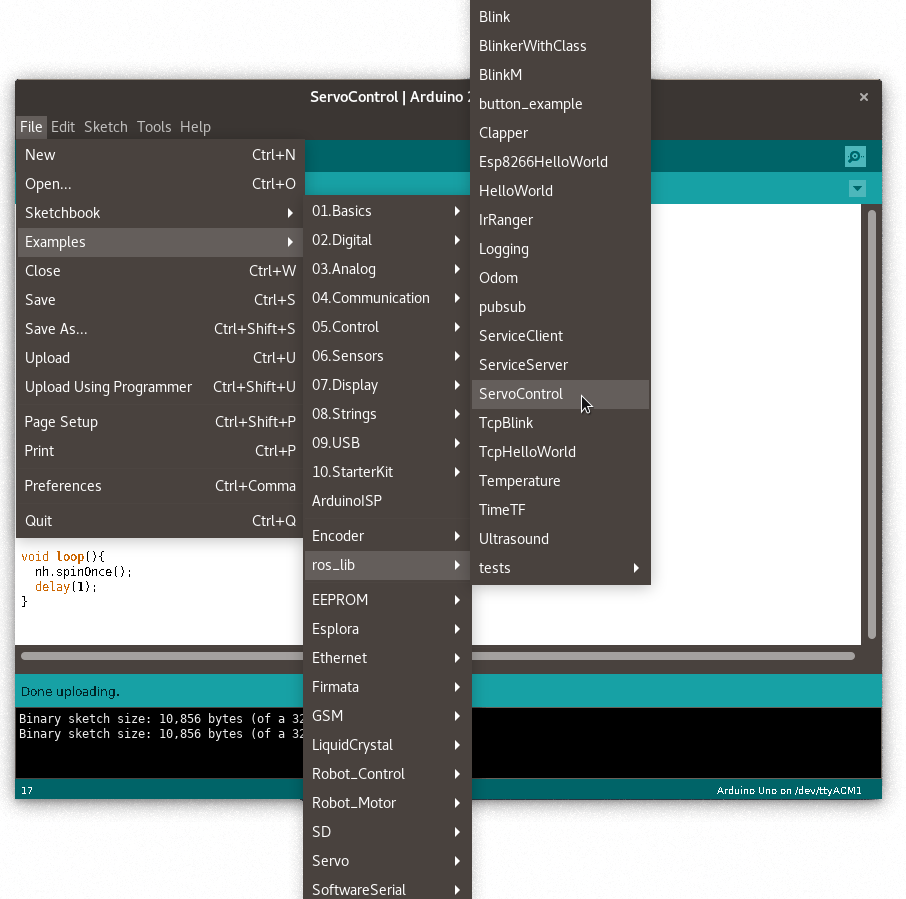
\includegraphics[width=0.9\linewidth]{arduino-ide-ros}
    \caption{Examples of ROS nodes for the Arduino}
    \label{}
\end{figure}


\step{Write a ROS node for your Arduino}


Use the following code sample to control a servo by sending one integer between
0 and 180:

\begin{cppcode}
#include <ros.h>
#include <std_msgs/UInt16.h>
#include <Servo.h> 

using namespace ros;

NodeHandle  nh;
Servo servo;

void cb( const std_msgs::UInt16& msg){
  servo.write(msg.data); // 0-180
}

Subscriber<std_msgs::UInt16> sub("servo", cb);

void setup(){
  nh.initNode();
  nh.subscribe(sub);

  servo.attach(9); //attach it to pin 9
}

void loop(){
  nh.spinOnce();
  delay(1);
}

\end{cppcode}

Compile and upload the code to the Arduino.

In a terminal, start \sh{rosserial} (setting the serial port as required):

\begin{shcode}
> rosrun rosserial_python serial_node.py /dev/ttyACM0
\end{shcode}

Now, call \sh{rostopic pub} with the adequate parameter to move your servo-motor.

\part{3D model of your arm}

We now want to build a 3D model of the arm. We first have to create a geometric
and kinematic description of the arm using the URDF format.

\step{Visualise a URDF file in RViz}

Create a new directory called \sh{robot-project} and a sub-directory called
{models}. Save the following URDF file in this subdirectory as
\sh{robot-arm.urdf}:

\begin{xmlcode}
<?xml version="1.0"?>
<robot name="roco_arm">
  <link name="base_link">
    <visual>
      <geometry>
        <cylinder length="0.06" radius="0.1"/>
      </geometry>
    </visual>
  </link>

  <link name="first_segment">
    <visual>
      <geometry>
        <box size="0.6 0.05 0.1"/>
      </geometry>
      <origin rpy="0 0 0" xyz="-0.3 0 0" />
    </visual>
  </link>

  <joint name="base_to_first" type="revolute">
    <axis xyz="0 1 0" />
    <limit effort="1000" lower="0"
                    upper="3.14" velocity="0.5" />
    <parent link="base_link"/>
    <child link="first_segment"/>
    <origin xyz="0 0 0.03" />
  </joint>
</robot>
\end{xmlcode}

Load this file as the \emph{description} of your robot: 

\begin{shcode}
> rosparam set robot_description -t models/robot-arm.urdf
\end{shcode}

Next, launch the \sh{robot_state_publisher} node:

\begin{shcode}
> rosrun robot_state_publisher robot_state_publisher
\end{shcode}

This node reads the robot description, and broadcasts the 6D transformations (TF
frames) corresponding to each of the links described in the URDF file.

Finally, add the \texttt{Robot model} plugin to RViz and set the \texttt{Fixed
frame} to \sh{/base_link}:


\begin{figure}[h!]
    \centering
    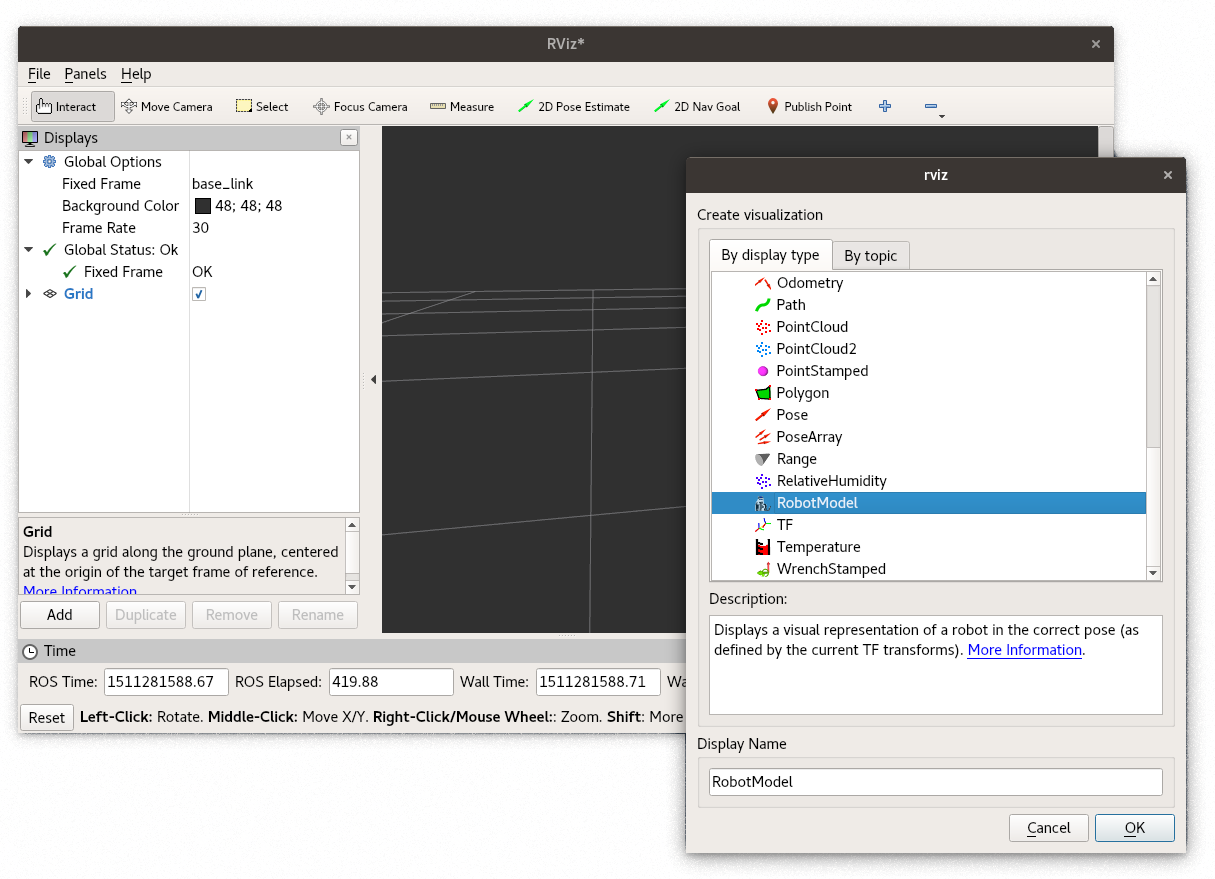
\includegraphics[width=0.9\linewidth]{rviz-plugins}
    \caption{Adding the \texttt{Robot model} visualisation plugin to RViz}
    \label{}
\end{figure}

You should see the following model in the 3D viewport:

\begin{figure}[h!]
    \centering
    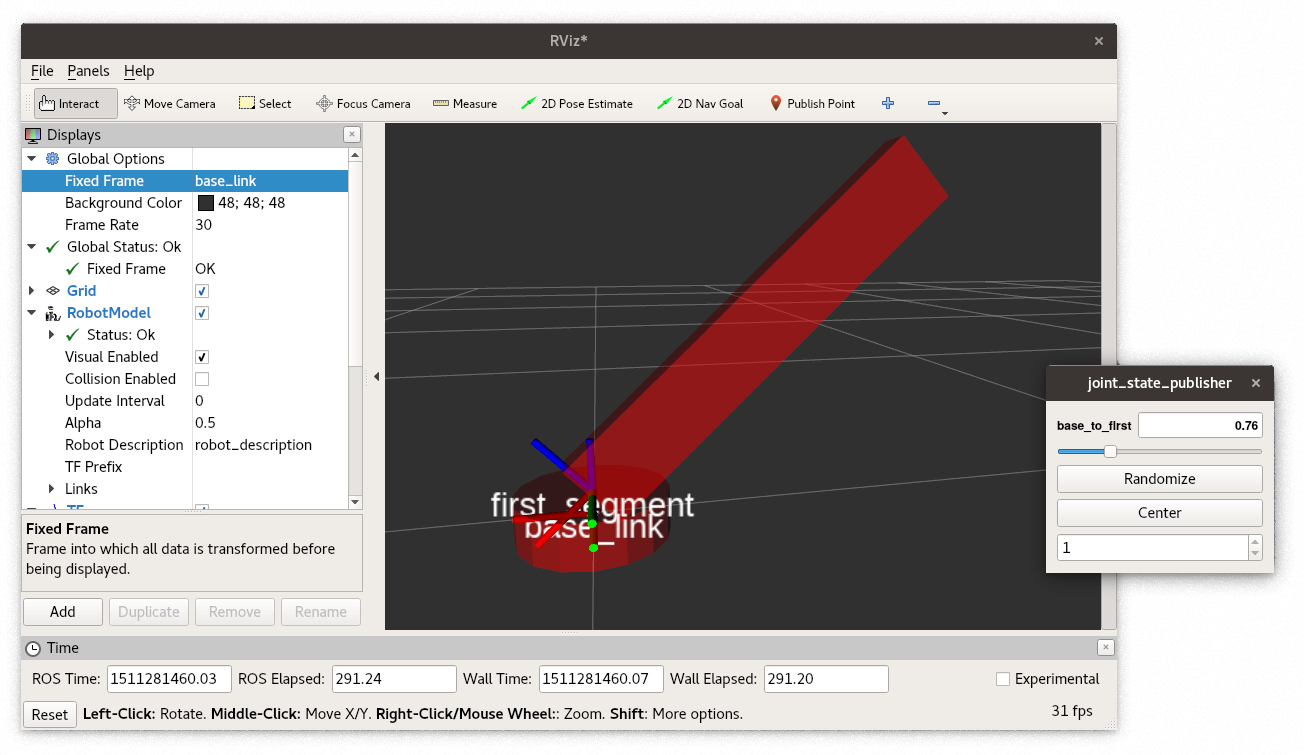
\includegraphics[width=0.9\linewidth]{urdf-rviz}
    \caption{A first, simple, URDF model, visualised in RViz.}
    \label{}
\end{figure}


\step{Create the URDF file of your robot}

Using \sh{robot-arm.urdf} as a starting point, complete the URDF to accurately
model your arm. Measure precisely the dimension of each segment, and place
accurately the joints.

If you wish to check your model, reload the robot description, and restart the
\sh{robot_state_publisher} node. You do not need to restart RViz, but you need
to desactivate and re-activate the \texttt{robot model} plugin to update the
rendering.

\more{
    Instead of simple geometric primitive, you can use STL meshes (like the ones
    you 3D printed) for the visuals of your arm. Check the
    \href{http://wiki.ros.org/urdf/XML/link}{URDF documentation} to learn how to
    do that.
}

\begin{shcode}
> rosrun joint_state_publisher joint_state_publisher _use_gui:=true
\end{shcode}


\note{
Document your findings with photographs and a short video of RC servo
operation.
}



\end{document}



